\chapter{OpenCAL OpenCL version}\label{ch:opencal-cl}


This chapter introduces OpenCAL-CL, a porting of OpenCAL in
OpenCL. OpenCL is a parallel framework originally proposed by Apple
and then released as an Open Standard under the Khronos Group
management. Besides computational efficiency, one of the main
advantages of OpenCL is portability. In fact, you can run your program
wherever you want across heterogeneous processors like Central
Processing Units (CPUs), Graphics Processing Units (GPUs), Digital
Signal Processors (DSPs), and Field-Programmable Gate Arrays (FPGAs).

OpenCAL-CL inherits many OpenCAL's features, by also adding parallel
computation capability thanks to the adoption of OpenCL. The
application is now subdivided in two parts: the \emph{host program},
running on the CPU, and the \emph{device program}, running on a
compliant computational device (e.g. an Nvidia or AMD GPU). The CA
object is still defined host-side, as in OpenCAL, while elementary
processes (and possibly other functions) are defined
device-side. Belonging to the device program, CA elementary processes
must be defined as OpenCL's \emph{kernels} and therefore the
programmer has to be able to write some minimal OpenCL code to
implement them. Fortunately, OpenCAL-CL hides lots of parallel aspects
to the user (e.g. the simulation loop is internally managed by the
library) and also simplifies data exchange between host and
device. The user’s OpenCL parallel programming background can be
therefore limited or even null. In the latter case, the user can learn
some basic elements of OpenCL kernel programming thanks to this guide.

This chapter is divided into two parts: the first part is a very brief
overview of OpenCL, while the second one introduces OpenCAL-CL by
examples.

\section{OpenCL framework}\label{sec:openclstructure}
OpenCL enables parallel programming that assigns computational tasks
to multiple processing elements to be performed at the same
time. These tasks are called \emph{kernels}. A kernel is a special
function that can be executed to different OpenCL-compliant
devices. In the CA modeling context, each elementary process of the CA
transition function is devised in the OpenCAL library as a kernel.  The kernels are sent
to the device(s) by the host application. The host application defines
a structure called \emph{context}, needed to manage data exchange and
computation on the compliant devices.

In particular, host application links kernels into one or more
programs. In the host application, the user can select the kernel's
functions to insert inside a container called \emph{program}.  The
program connects the kernel with argument data and dispatches it to a
structure called \emph{command queue}.  The command queue is a structure that
allows the host to decide what the devices have to do and, when a
kernel is enqueued, the device will execute the relative function.

\begin{figure}[htp]
  \begin{center}
    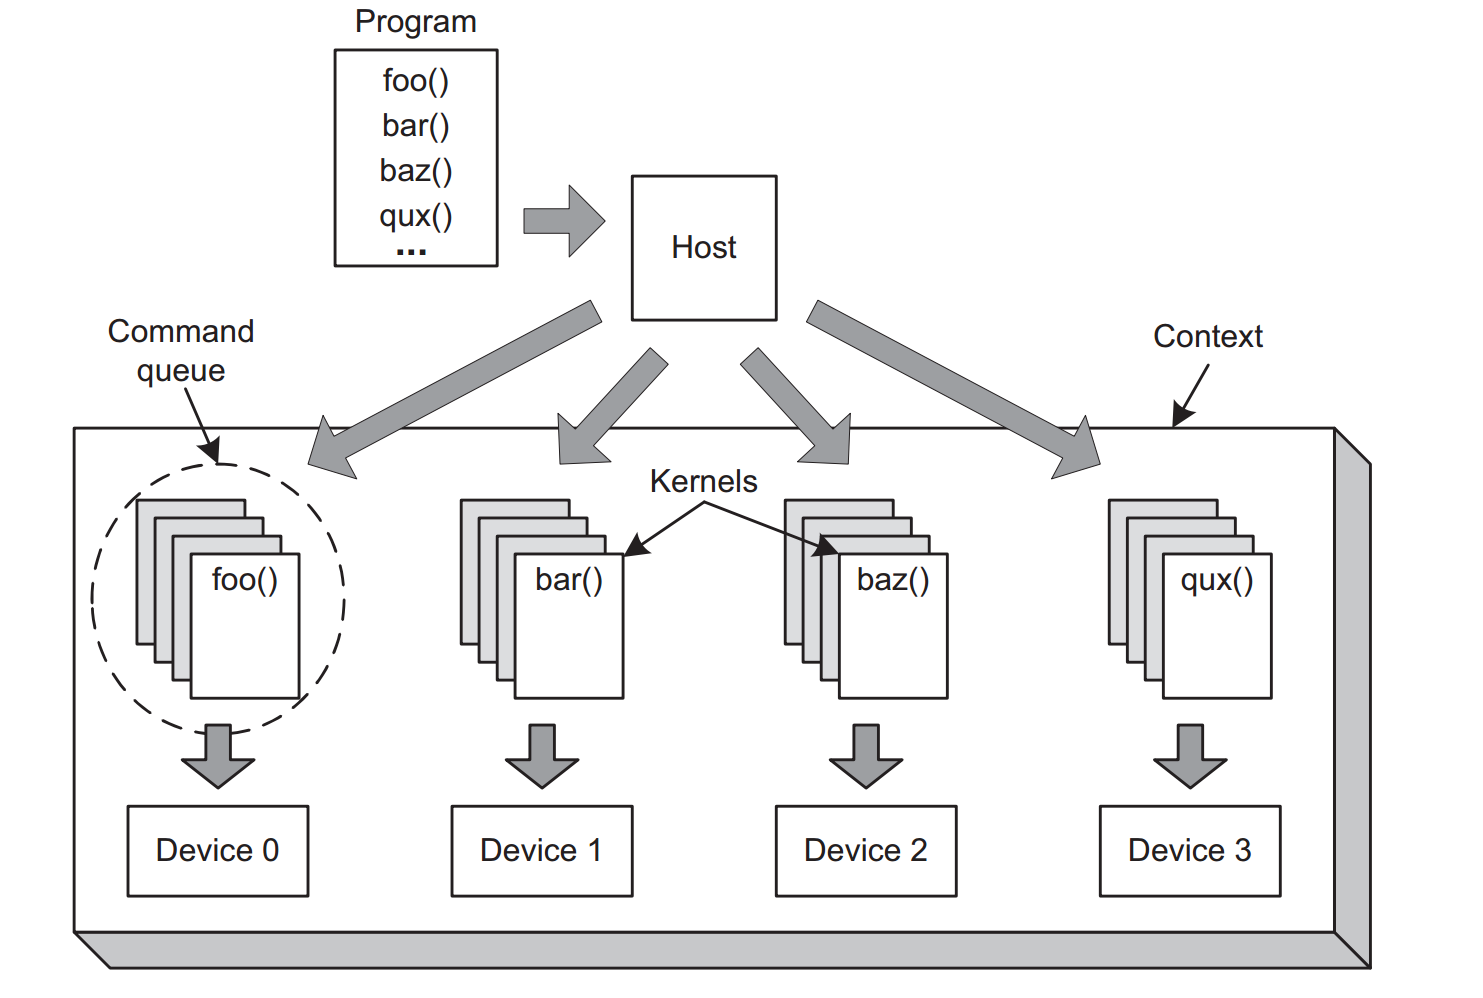
\includegraphics[width=12cm]{./images/OpenCAL-CL/kernelDistribution}
    \caption{General structure of a OpenCL program}
    \label{fig:GeneralStructure}
  \end{center}
\end{figure}

As we can see from the picture above, the context contains all the
devices, all the command queues and all the kernels.  More in detail,
for every device a command queue is associated and every command queue
has inside all the kernel functions that the device has to execute.

\section{The structure of OpenCAL-CL}
As in OpenCL applications, the OpenCAL-CL library has a set of
structures and functions to develop host program and to define
kernels. The definition of the CA is specified in the host
program. The user can define two types of models, 2D or 3D, as shown
in \ref{ch:opencal}.  The host program manages the kernels and
dispatches the data of the mode (e.g., CA substates, the type of
neighbourhood, size of the cellular space, etc) to the computation
units.  The host program manages the execution loop and which
computation unit has to execute the transition functions. \\ The host
program is typically divided in the following sections:
\begin{itemize}
\item definition of the model (Chapter \ref{ch:opencal})
\item management of the OpenCL devices
\item kernels allocation
\item data dispatch from the model to devices
\item execution loop start
\end{itemize}

\section{Host programming} 

\subsection{Definition of the model}

XXX

\subsection{Manage of the devices}

After the model creation, the user must choose the device for the
kernel computation.  Inside the library, a structure called CALOpenCL
allows the user to manage all available platforms and devices.  This
structure simplifies the access to the devices compared with the
native API of OpenCL. The library supplies other functions to know
which platforms and devices are available on the system and to have
information about these.\\ Below you can see a simple program that
explains how the CALOpenCL structure can be used.


\begin{lstlisting}
#include <calCL2D .h>

 int main (){

 CALOpenCL * calOpenCL = calclCreateCALOpenCL (); // get all available
 platforms calclInitializePlatforms ( calOpenCL ); // get all
 available devices calclInitializeDevices ( calOpenCL );

 // get the first device on the first platform CALCLdevice device =
 calclGetDevice ( calOpenCL , 0, 0);

 // create a context CALCLcontext context = calclcreateContext (&
 device , 1);

 return 0; }
\end{lstlisting}

Inside the library, the platforms and the devices are stored in a
matrix where rows represent the platforms and columns represent the
devices. Thus, to choose which one we can use for the computation,
it is necessary to specify the index of platform and the index of the
device. For example, at lines 12, we chose the platform number 0 and
the device number 0. If we have a system with 3 NVIDIA GPUs and 3 AMD
GPUs, the library will have a $2 \times 3$ size matrix, where 2 are the vendors
(i.e., the platforms NVIDIA and AMD) and 3 are the GPUs for each
platforms. If we want to run the program using the third AMD GPU, we can
specify 1 and 2 as indices. If we don't know how the system identifies
the platforms and devices, the library supplies us a function called
\verb'calclGetPlatformsAndDeviceFromStandardInput' that allows us to
know the available platforms and devices. First it prints the information on
standard output and then we can insert the indexes directly from
standard input.\\ After the device is chosen, the user must specify the
path where the kernels and relative headers are. Through the function
\verb'calclLoadProgramLib(2D/3D)' the library reads automatically the
kernels and compiles them.

\begin{lstlisting}
CALCLprogram calclLoadProgramLib(2D|3D) ( CALCLcontext context ,
CALCLdevice device , char * path_user_kernel , char *
path_user_include )
\end{lstlisting}

\subsection{Allocation of kernels}

The library doesn't know which kernels are related to the CA elementary
processes, nor their execution order on the available devices.  Thus, to create and allocate a kernel it's necessary
to call the function \verb'calclGetKernelFromProgram' that retrieves an
OpenCL kernel given a compiled OpenCL program.

\begin{lstlisting}
cl_kernel elementaryProcess = calclGetKernelFromProgram(&program,
KERNEL_NAME);
\end{lstlisting}


\subsection{Send data from the model to devices}

To transfer the data from host side to kernel side, the user must
define the structure called \verb'CALCLToolkit(2D/3D)' containing all
the buffers (data) of the model.  By default, the library sends to all
the kernels the data associated to the model. The following list shows
the data which is sent:
\begin{itemize}
	\item the dimension of cellular space
	\item the number of substate for every type (i.e., byte, int, real)
	\item the substates allocated from the user
	\item the list of active cells
	\item the list of active cells flags
	\item type, dimension and ID of the neighbourhood
	\item the border condition
\end{itemize}


 First, the user must create an instance of the structure
 \verb'CALCLToolkit(2D/3D)' by calling the function
 \verb'calclCreateToolkit' as shown in the following code snippet.

\begin{lstlisting}
CALCLToolkit2D * calclCreateToolkit (2D|3D)(struct CALModel (2D|3D)
*model ,CALCLcontext context ,CALCLprogram program ,CALCLdevice device
,CALCLOptimization opt)
\end{lstlisting}

The enumerative \verb'CALCLOptimization' allows the user to choose if
she/he wants to use the library without optimization \verb|(CALCL_NO_OPT)|
or with active cells optimization \verb|(CALCL_OPT_ACTIVE_CELLS)|. The
structure \verb'CALCLToolkit(2D/3D)' doesn't contain only the buffers
to transfer data but also the kernels belonging to the execution
loop. \\ To add a new kernel to the execution loop, the user has to
call the function \verb'calclAddElementaryProcessKernel(2D/3D)' that
adds the chosen kernel to the list of CA elementary processes; moreover, it
sends to the device all the necessary data to execute the kernel.

\begin{lstlisting}
void calclAddElementaryProcessKernel2D(CALCLToolkit2D * toolkit2d,
struct CALModel2D *model, CALCLkernel * elemProcKernel);
\end{lstlisting}


\subsection{Start execution loop}

To start the execution loop, the user has to call the function
\verb'calclRun(2D/3D)'. This function executes all the elementary
processes previously declared on the specified device.

\begin{lstlisting}
void calclRun2D(CALCLToolkit2D* toolkit2d, struct CALModel2D * model,
unsigned int initialStep, unsigned maxStep);
\end{lstlisting}


\section{Kernel programming} 

In order to program kernels in OpenCAL, the user needs to include some header files.
Specifically, cal2D.h or cal3D.h permit to use some simple
functions to interact with the data structures belonging to the model.
To create a kernel function in OpenCL, user must place the keyword
\verb'__kernel' before the returning the type of the function. In
OpenCAL-CL every time a kernel function, the keyword \verb'MODEL_DEFINITION2D' must be specified as first parameter and the
function \verb'initThreads2D()' called as first instruction.\\ The code below
shows how to declare a new kernel.

\begin{lstlisting} 
__kernel void kernel(MODEL_DEFINITION2D){ initThreads2D(); ...  ...
    ...  }
\end{lstlisting}

When the user implements an elementary process - by defining
its kernel function - she/he can rely on a set of OpenCAL functions
that allow to get the substates values of both the central and the
neighbouring cells, and to update the substates values of the central
cell. Every time the user wants to use this function, the keyword \verb'MODEL2D' must be passed
as first parameter. For instance, if we
want to retrieve the value of a specific cell we need to use the function
\verb'calGet2Dr'.

\begin{lstlisting} 
	double a = calGet2Dr(MODEL2D, 0, i, j);
\end{lstlisting}

The function returns the value of the cell (i, j) of the substate 0.\\ Since inside OpenCAL-CL one can use all OpenCL features, all memory levels such as global memory, local memory, private
memory (XXXcitazione libroXXX) can be exploited. In order to use these memory levels, variables must be declared using this specific syntax respectively
\verb'__global', \verb'__local', \verb'__private'.

\subsection{Conway’s Game of Life}
 
As already reported in \ref{sec:cal_life}, to introduce how to develop a
Cellular Automata model with OpenCAL-CL we can start by implementing Conway’s
Game of Life and specifically its host application part. In order to use OpenCAL-CL, some
header files are included (lines 3-8) and, in particular, the OpenCAL library and
the OpenCAL-CL library. The OpenCAL library
inclusion inside the host application is necessary to define the CA object
(line 46) and the related substate (line 49). The cal2DIO.h header
file (line 4) provides some basic input/output functions for
reading/writing substates from/to file. To run the application with
OpenCAL-CL, all the necessary objects have to be declared (line
27-31). Respectively, the following variables have to be declared: the
\verb'CALOpenCL' structure (line 27), the \verb'CALCLcontext', the
\verb'CALCLdevice', the \verb'CALCLprogram' and the
\verb'CALCLToolkit2D'.  To create and initialize these variables we
need to call the function \verb'calclCreateCALOpenCL' that creates the
CALOpenCL structure, the functions \verb|calclInitializePlatforms| and
\verb|calclInitializeDevices| to initialize all the platforms and
devices on the available machine and the function \verb'calclGetDevice()', which
will return the device where elementary process are computed by
choosing the integers \verb'platformNum' and \verb'deviceNum' (line
24-25).  Morevoer, two important functions which are considered are \verb'calclcreateContext'
and \verb'calclLoadProgramLib2D'.  The first returns the context
\ref{sec:openclstructure}, while the second builds all kernels inside the
path specified by \verb'kernelSrc'(line 15) including the files
specified by \verb'kernelInc'(line 16), returning a program
containing all the compiled kernels.

\lstinputlisting[label=lst:cal_sciddicaT, caption=An OpenCAL-CL
  implementation of the Conway's game of
  Life.]{../opencal/OpenCAL-CL/examples/calcl_life/source/life.c} Here
you can see the device code of the Conway’s Game of Life:
\lstinputlisting[label=lst:cal_sciddicaT, caption=An OpenCAL-CL kernel
  to implement the Conway's game of Life elementary
  process.]{../opencal/OpenCAL-CL/examples/calcl_life/kernel/source/life.cl}
 
